\section{Demo}
\label{demo}

In this section, we describe how to run the project demo and get started with the simulation of the Raft protocol.

\subsection{Requirements}

The following requirements must be met in order to run the project:

\begin{itemize}
    \item Java 17.0.1 (or later)
    \item Apache Maven 3.8.4 (or later)
\end{itemize}

Project dependencies (such as JavaFX) are managed by Maven, and will be pulled and installed once the project is imported and set up. At the moment, we do not provide an executable \verb=jar= file.

To get started, obtain the source code from the GitHub repository:

\begin{verbatim}
    git clone git@github.com:andreastedile/raft-simulator.git
\end{verbatim}

Then, move into the directory, and use Maven to start the project:

\begin{verbatim}
    mvn javafx:run
\end{verbatim}

Maven stores all the information about the project in the \verb=pom.xml= file, which is available in the project root. This includes the JavaFX plugin, which enables Maven to automatically link JavaFX libraries with the compiled Java code.

Once the aformentioned command is run, Maven will query the repository, pull the relevant dependencies, build the project, and finally open a pop-up Java window, as in \autoref{fig:raft-start}.

\subsection{The GUI}

\begin{figure}[ht]
    \centering
    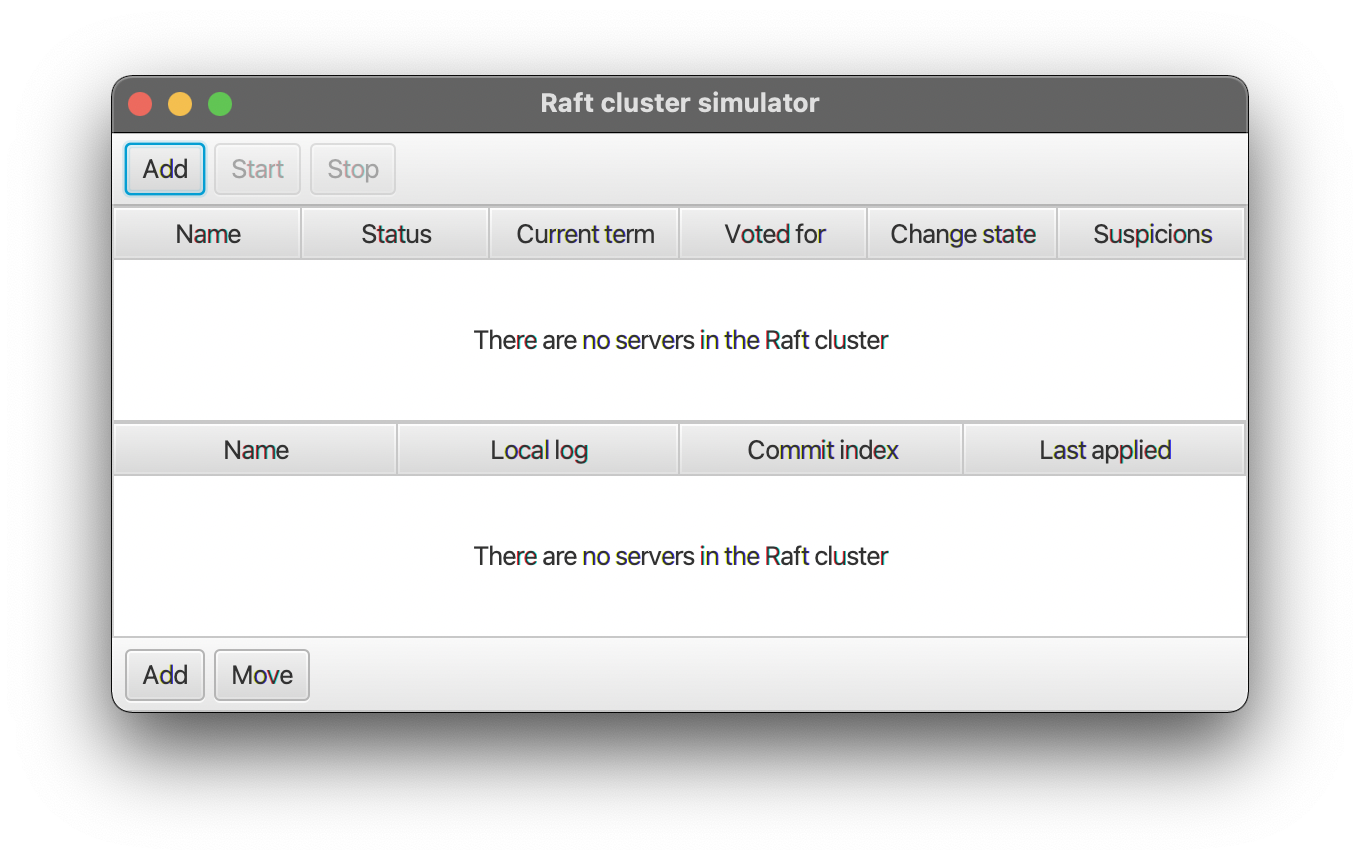
\includegraphics[width=0.66\textwidth]{drawable/init-page.png}
    \caption{The Raft simulator window at start.}
    \label{fig:raft-start}
\end{figure}

The GUI is composed of three sections: the \textit{toolbar}, the \textit{server view}, and the \textit{log view}.

The \textit{toolbar} sits at the top of the window, and is the entrypoint for starting the Raft cluster. It has three buttons, which are dynamically enabled and disabled depending on the context. To get started, press the \textit{Add} button to add a Raft server. Repeat until a satisfactory number of servers is inserted in the system. Note that, once a server has been added, it cannot be removed.

Once at least a server is added to the cluster, the \textit{Start} button is enabled, allowing the system to be started. Since one of the assumptions of the Raft protocol is that the number of servers in the cluster shall not change, once the simulation is started adding more servers is not supported, and the relevant button is grayed out.

In the \textit{server view}, a sortable list of servers is populated as the \textit{Add} button is repeatedly clicked. Fields presented included the name, the status (\texttt{FOLLOWER}/\texttt{CANDIDATE}/\texttt{LEADER}), the current term, and who the server voted in this term. Finally, a button is available on the far right of each right. \autoref{fig:adding-server} shows an example of the GUI once some servers are added.

\begin{figure}[ht]
    \centering
    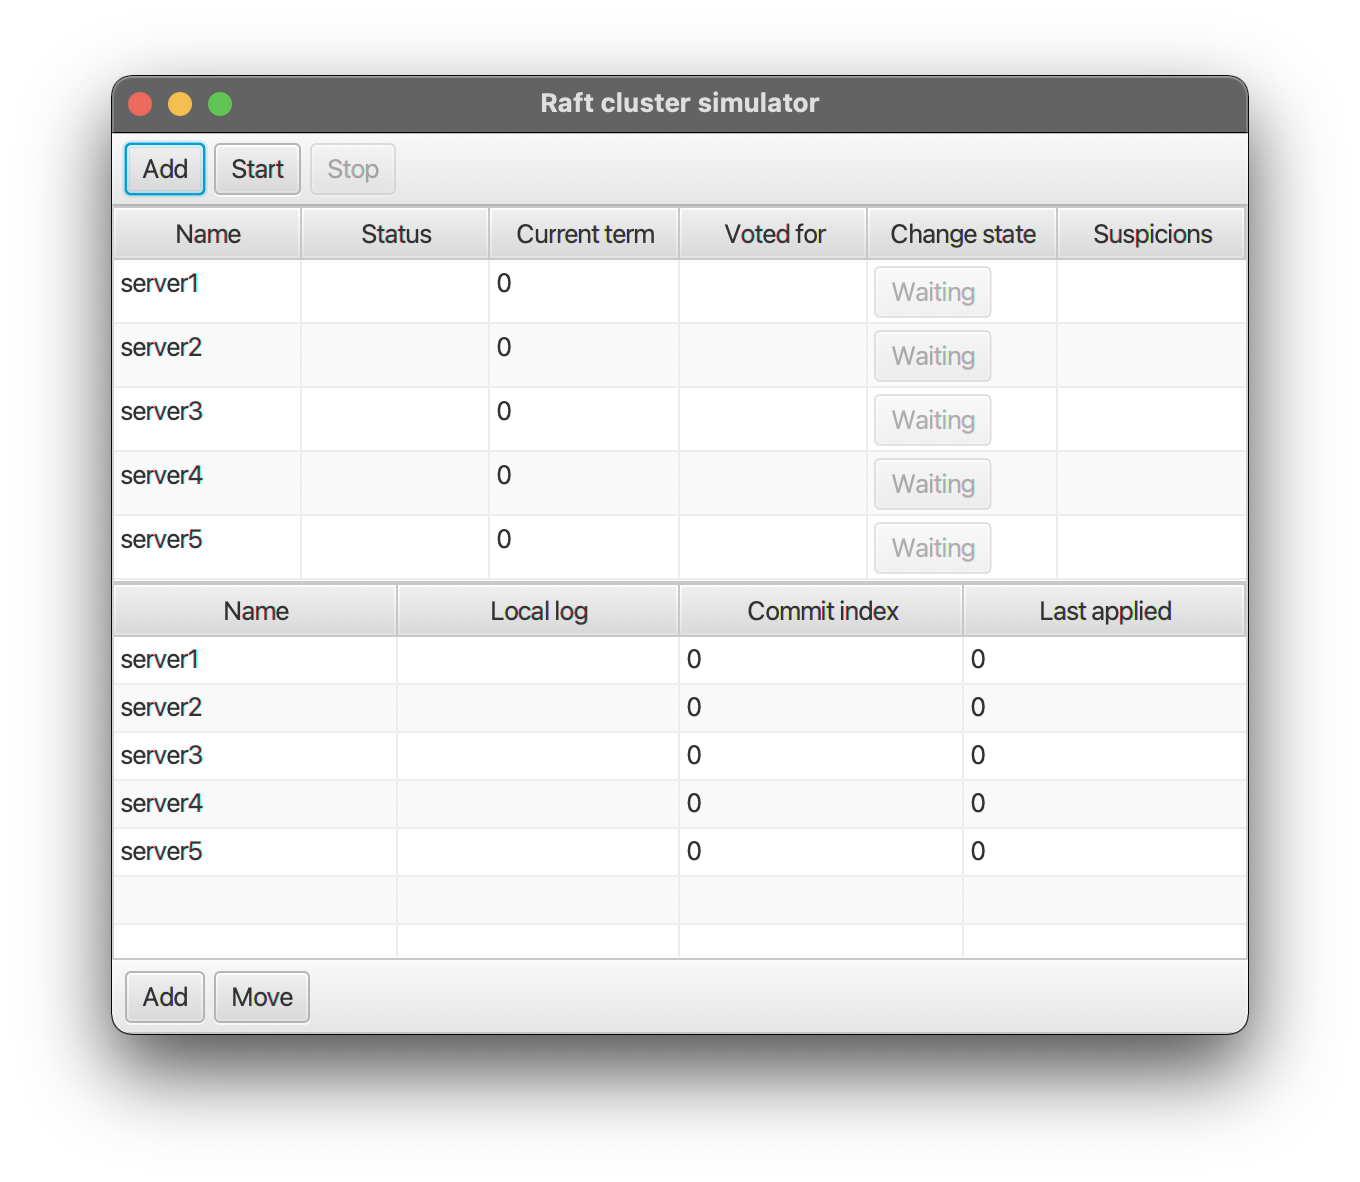
\includegraphics[width=0.66\textwidth]{drawable/adding-few-servers.png}
    \caption{Adding a handful of servers to the simulation.}
    \label{fig:adding-server}
\end{figure}

This button, which is active only when the simulation has been started, allows the user to programmatically crash the related node. The node will stay in a crashed state (i.e. will ignore any incoming message and forget its non-persistent state) until the user presses the button again, effectively rebooting it.

On the bottom \textit{log view}, another table is available which shows the local log, the commit index, and when the commit was last applied. Two additional buttons are available, which allow the user to query the current leader and ask to add an entry to the log.

\subsection{Starting the simulation}

\begin{figure}[ht]
    \centering
    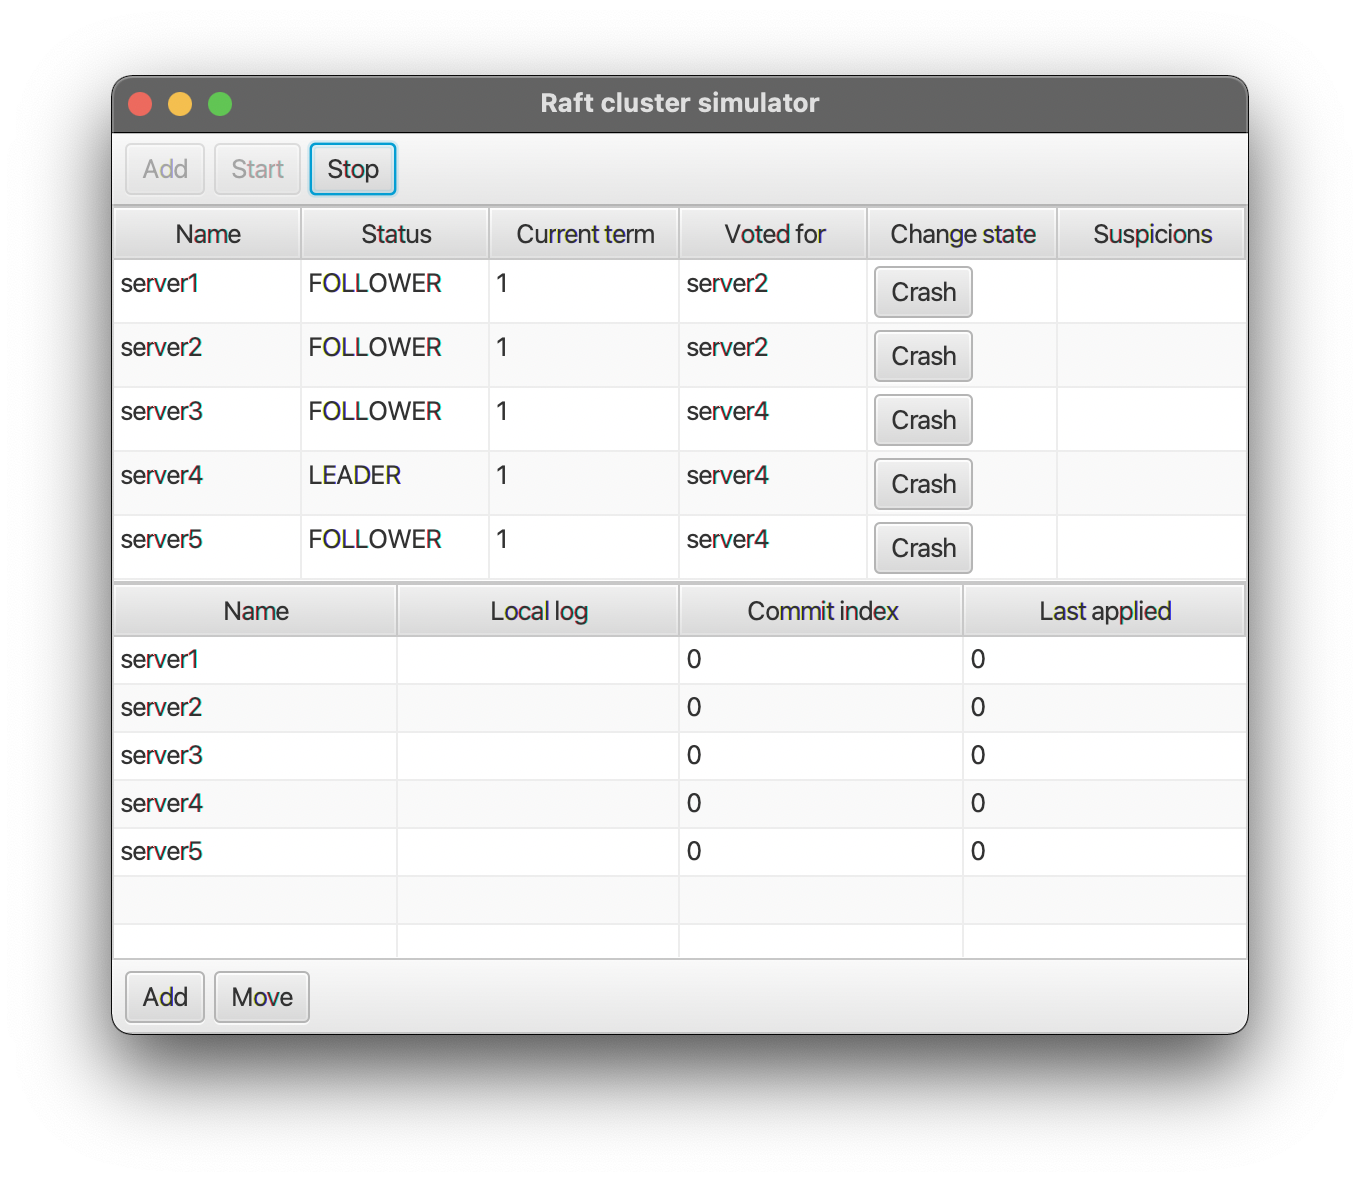
\includegraphics[width=0.44\textwidth]{drawable/1-starting-simulation.png}
    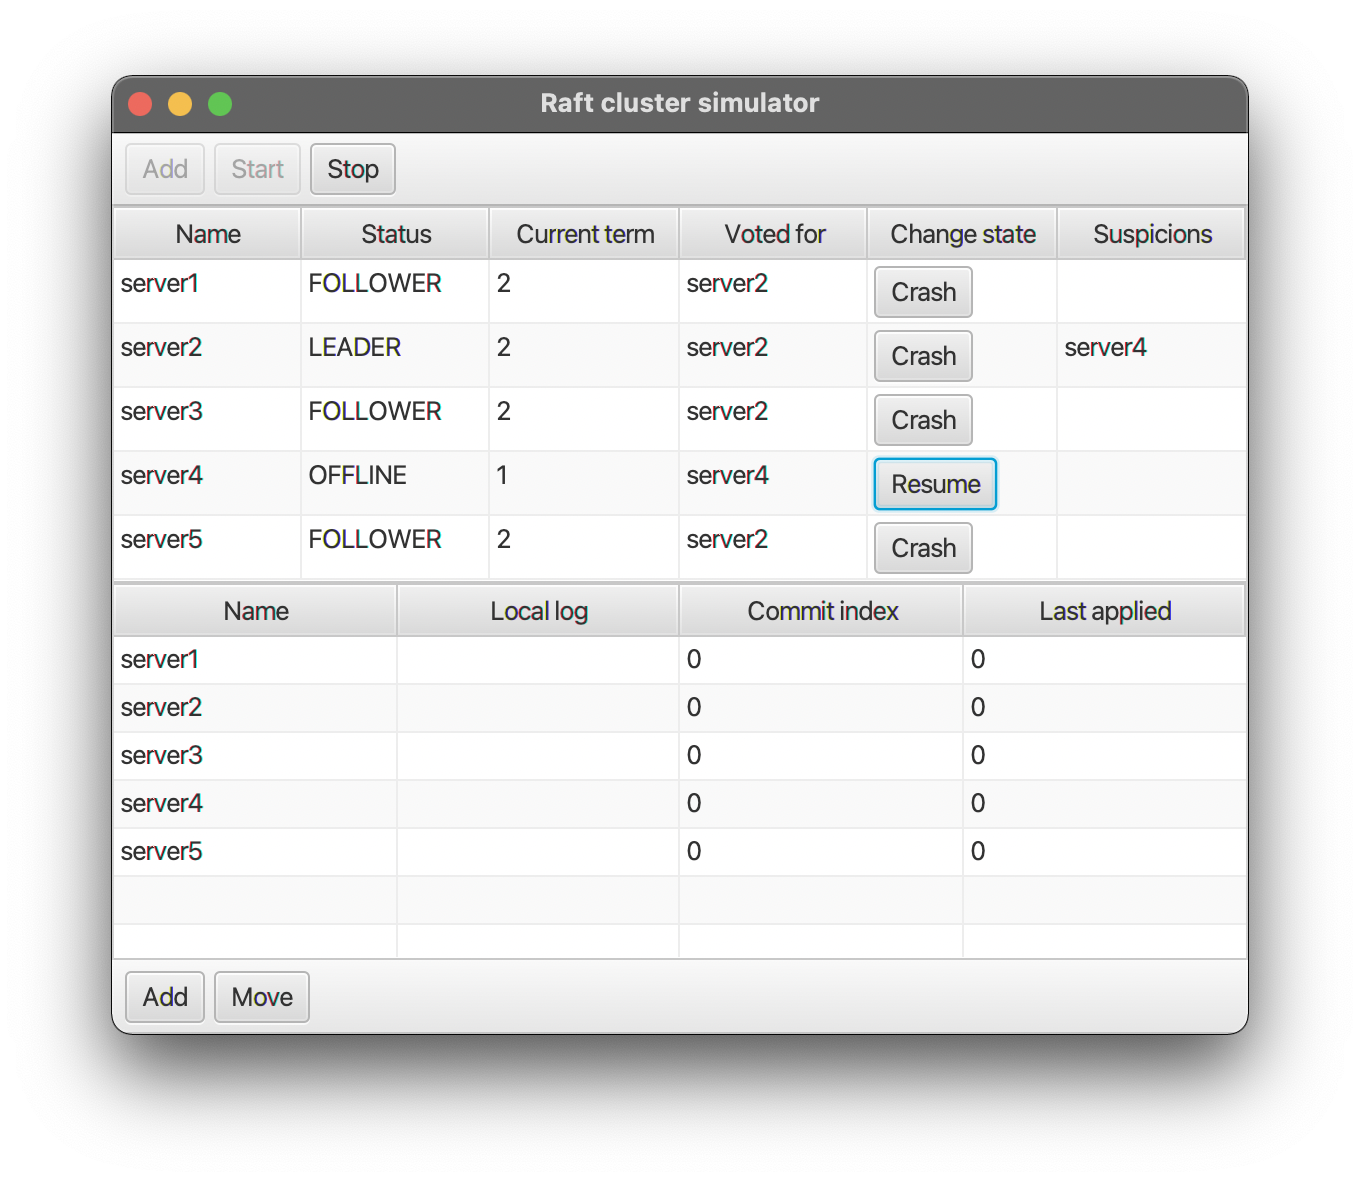
\includegraphics[width=0.44\textwidth]{drawable/2-crashing-leader.png}
    
    \caption{The start of the simulation, and crashing the current leader.}
    \label{fig:starting-simulation-crash}
\end{figure}

Once the user is satisfied with the amount of servers added to the simulation and has started it, the Raft cluster will let every server know each other and let them interact freely using the primitives described in \autoref{architecture}. The servers will set an \texttt{electionTimeout}, and after a short time, one will prevail and will be elected leader. For showcasing purposes, we can crash it with its button. \autoref{fig:starting-simulation-crash} shows an example of what happens in the GUI: as the leader is killed, the other servers' timeouts will expire and will elect a new leader, as they will still be able to meet the majority criteria.


\begin{figure}[ht]
    \centering
    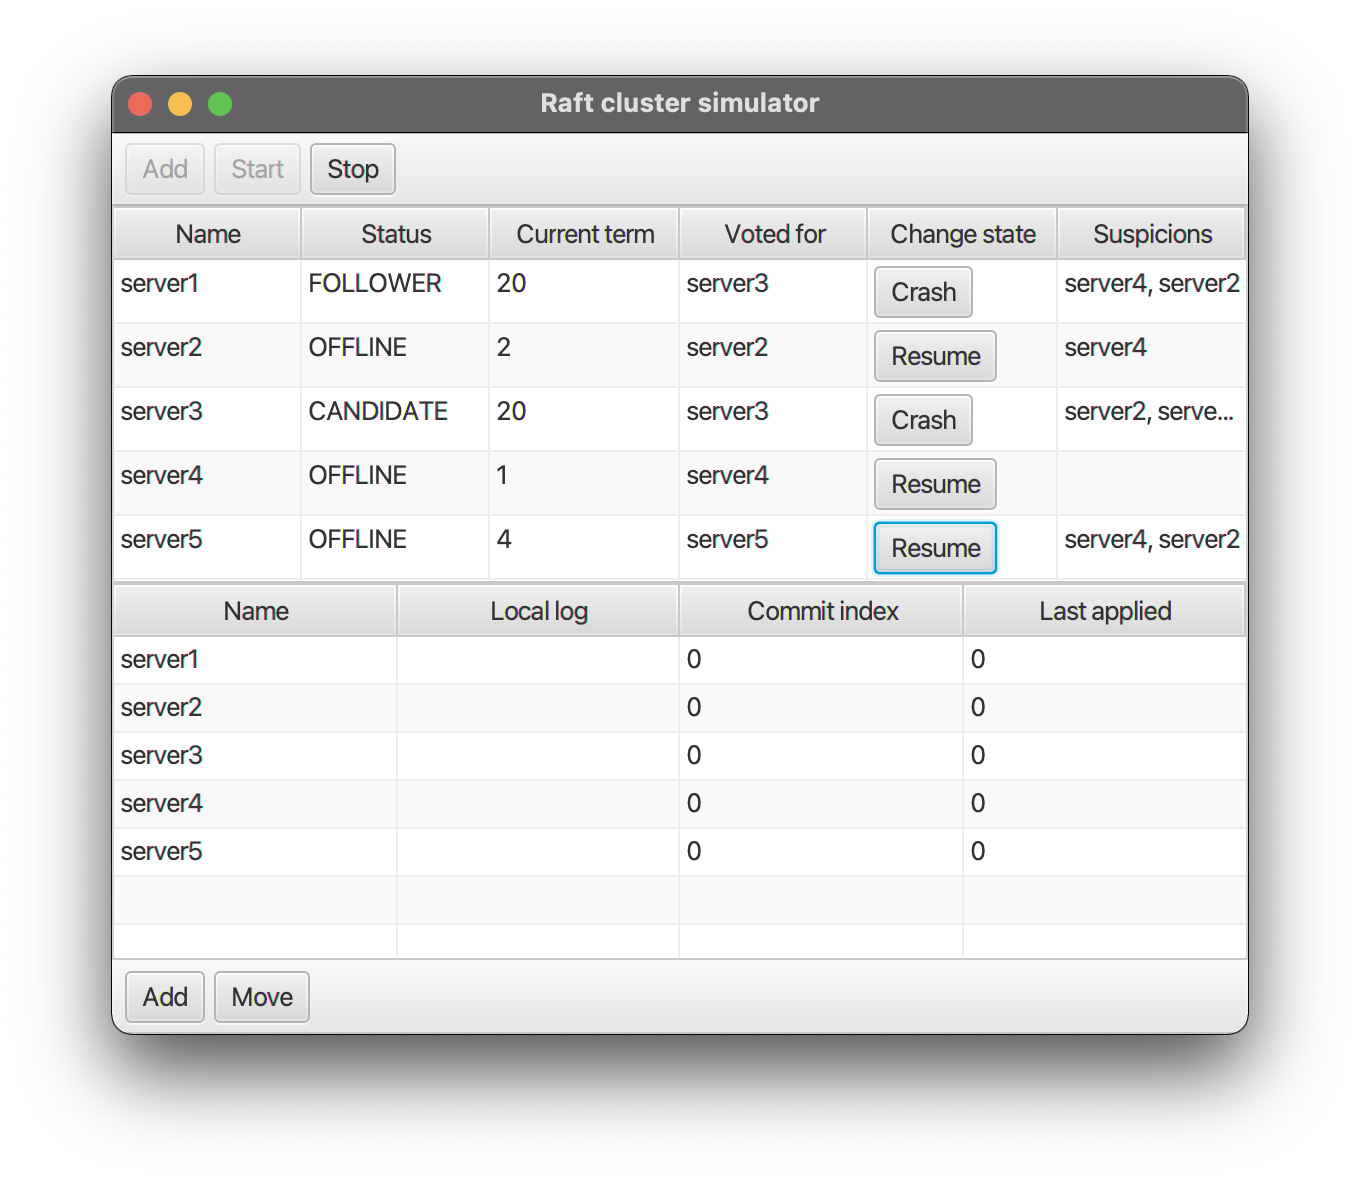
\includegraphics[width=0.44\textwidth]{drawable/2a-chaos-leader.png}
    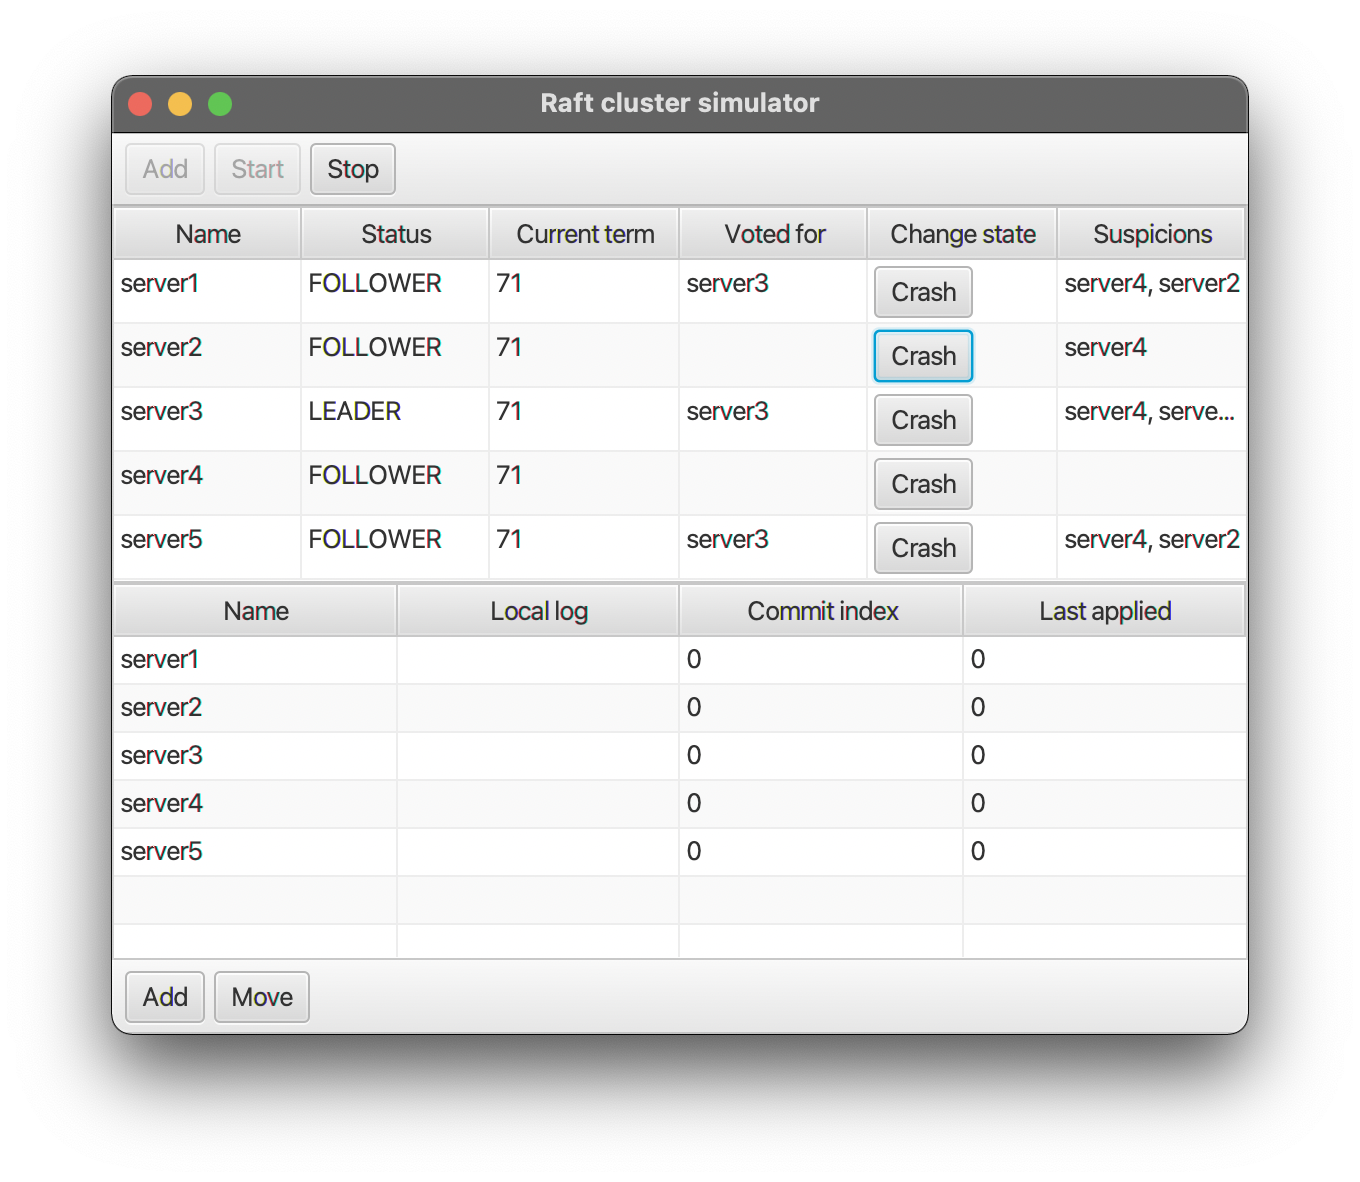
\includegraphics[width=0.44\textwidth]{drawable/3-leader-comeback.png}
    
    \caption{Crashing more than the majority of the servers: to the left, terms start increasing drammatically. To the right, term parity is achieved when they resume from the crash.}
    \label{fig:crash-comeback}
\end{figure}

If the user were to crash more than the majority of the servers, then the remaining servers will start panicking and, as their election timeouts repeatedly expire, start increasing their terms. \autoref{fig:crash-comeback} (left) shows an example of this effect. This is expected behavior, as two servers out of five should never be able to elect a new leader. On the other hand, \autoref{fig:crash-comeback} (right) shows the result of a clean comeback from a crash. The previous leader (\texttt{server2}) came back and was swiftly deposed by the new one, and with the \texttt{appendEntries} messages was informed of the new term and leader. We can observe that \texttt{server2} did not vote for anyone in this term. Again, this is to be expected, as the server was crashed during the election.

\begin{figure}ht
    \centering
    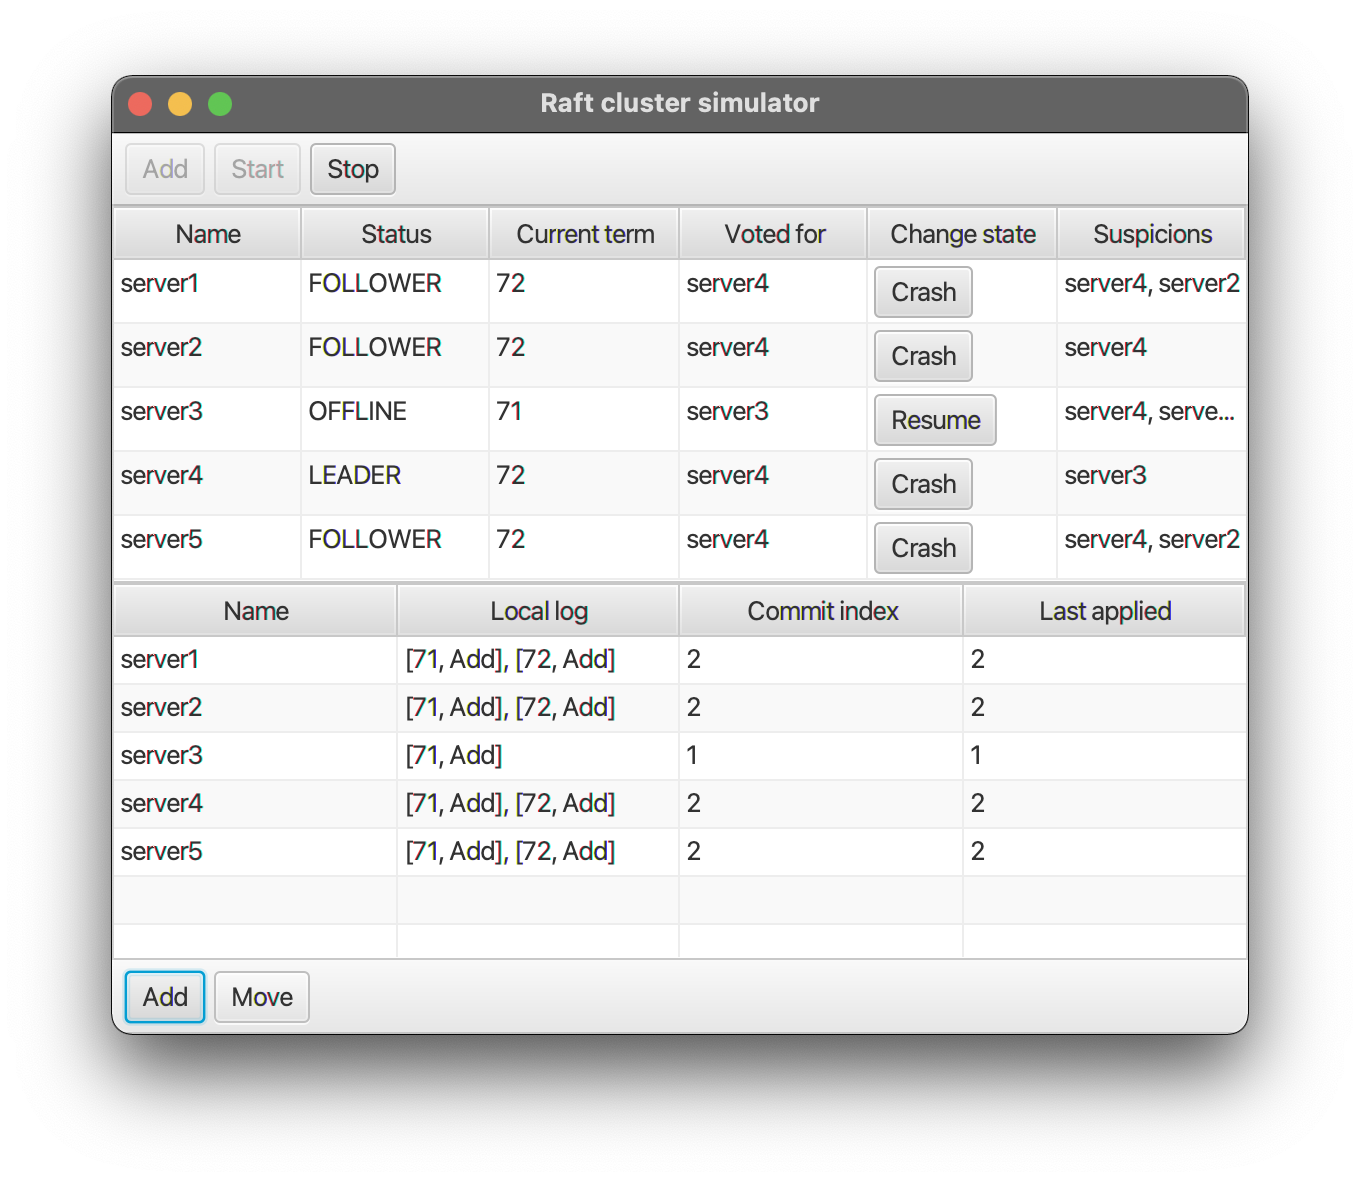
\includegraphics[width=0.66\textwidth]{drawable/4-some-logs.png}
    
    \caption{Adding some logs.}
    \label{fig:adding-logs}
\end{figure}

Finally, \autoref{fig:adding-logs} shows an example of an addition of log entries to the cluster. At first, all servers have recovered from the crashes in previous screenshots. One request is made to the leader of term 71 while all servers are alive. This results in a swift addition to each server's local log. Then, \texttt{server3} is crashed, and an additional request is made to the new leader. Now, every server but \texttt{server3} is aware of the request and has applied it, as the majority was still met even without him. When \texttt{server3} will come back, he will learn with \texttt{appendEntries} messages of the new entries  and will update its local log accordingly.

\subsection{Simulation parameters}

The simulation supports fine tuning of some parameters. This is done via the \verb=simulation.properties= file. The provided file looks like this:

\begin{verbatim}
    timeScale=1
    minElectionTimeoutMs=150
    maxElectionTimeoutMs=800
    heartbeatMs=50
    rpcTimeoutMs=15
    maxCrashDuration=10
\end{verbatim}

The configurable parameters are as following:

\begin{itemize}
    \item \texttt{timeScale}: an integer $\ge 1$. It is used as a factor for other parameters, and allows slowing down the simulation;
    \item \texttt{minElectionTimeoutMs} and \texttt{maxElectionTimeoutMs}: the floor and ceiling values used by the PRNG when computing election timeouts after each \texttt{appendEntries} message;
    %\item \texttt{heartbeatMs}
    \item \texttt{rpcTimeoutMs}: the milliseconds waited by servers before retrying an RPC.
    %\item \texttt{maxCrashDuration}: the maxi
\end{itemize}

\clearpage
\newpage
